\documentclass[8pt,serif]{beamer}
\usetheme[
%%% options passed to the outer theme
%    hidetitle,           % hide the (short) title in the sidebar
%    hideauthor,          % hide the (short) author in the sidebar
%    hideinstitute,       % hide the (short) institute in the bottom of the sidebar
%    shownavsym,          % show the navigation symbols
%    width=2cm,           % width of the sidebar (default is 2 cm)
%    hideothersubsections,% hide all subsections but the subsections in the current section
%    hideallsubsections,  % hide all subsections
%    left                % right of left position of sidebar (default is right)
]{Aalborg}
\usepackage[utf8]{inputenc}
\usepackage[T1]{fontenc}

%\usefonttheme{professionalfonts}
% If you want to change the colors of the various elements in the theme, edit and uncomment the following lines
% Change the bar and sidebar colors:
%\setbeamercolor{Aalborg}{fg=red!20,bg=red}
%\setbeamercolor{sidebar}{bg=red!20}
% Change the color of the structural elements:
%\setbeamercolor{structure}{fg=red}
% Change the frame title text color:
%\setbeamercolor{frametitle}{fg=blue}
% Change the normal text color background:
%\setbeamercolor{normal text}{bg=gray!10}
% ... and you can of course change a lot more - see the beamer user manual.
\usepackage[activeacute,spanish,es-tabla]{babel} 
\usepackage{amsmath,amssymb,amsfonts,latexsym,stmaryrd,eucal,amsthm,textcomp,cancel,nicefrac}
\usepackage{fourier}
\usepackage{graphicx}
\usepackage{animate}
\usepackage{empheq,fancybox}
\usepackage{xcolor}
\usepackage{colortbl}
\usepackage{booktabs}
\usepackage{xfrac}
\spanishdecimal{.}
\usepackage{etoolbox}
\usepackage[listings,most]{tcolorbox}
\usepackage{ragged2e}
\usepackage[export]{adjustbox}
\usepackage{pgffor}
\usepackage{enumitem}
\usepackage{tabularx}
\usepackage{physics}



%%%%%%%%%%%%%%%%%%%%%%%%%%%%%%%%%%%  Ref Equations %%%%%%%%%%%%%%%%%%%%%%%%%%%%%%%%%%%%%%%%%%%%%
\usepackage[spanish]{cleveref}
\crefname{equation}{ecuación}{ecuaciones}
\Crefname{equation}{Ecuación}{Ecuaciones}
\crefname{table}{tabla}{tablas}
\Crefname{table}{Tabla}{Tablas}

\crefname{figure}{figura}{figuras}
\Crefname{figure}{Figuras}{Figuras}




%%%%%%%%%%%%%%%%%%%%%%%%%%%%%%%%%%% Beamer Options %%%%%%%%%%%%%%%%%%%%%%%%%%%%%%%%%%%%%%%%%%%%%
% \setbeamerfont{section in sidebar}{size=\fontsize{6}{5}\selectfont}
% \setbeamerfont{subsection in sidebar}{size=\fontsize{5}{5}\selectfont}
% \setbeamerfont{subsubsection in sidebar}{size=\fontsize{4}{5}\selectfont}
% \setbeamerfont{caption}{series=\mdseries,size=\tiny,family=\rmfamily}
\setitemize{label=\usebeamerfont*{itemize item}%
	\usebeamercolor[fg]{itemize item}
	\usebeamertemplate{itemize item}}
\setbeamertemplate{caption}[numbered]
\setbeamertemplate{bibliography item}{[\theenumiv]}
\setbeamertemplate{navigation symbols}{}

%\setbeamercolor{section in sidebar shaded}{fg=blue} 
% \setbeamercolor{subsection in sidebar}{bg=gc} 
% \setbeamertemplate{section in head/foot}{\hfill\insertsectionheadnumber.~\insertsectionhead}
% \setbeamertemplate{section in head/foot shaded}{\color{structure!50}\hfill\insertsectionheadnumber.~\insertsectionhead}
% \setbeamertemplate{section in toc}{\inserttocsectionnumber.~\inserttocsection}


% \makeatletter
% \patchcmd{\insertverticalnavigation}%
% {\ifx\beamer@nav@css\beamer@hidetext{\usebeamertemplate{section in sidebar}}\else{\usebeamertemplate{section in sidebar shaded}}\fi}%
% {{\usebeamertemplate{section in sidebar}}}{}{}
% \makeatother


% ----->  Some definitions

% Set up some colors
\definecolor{gc}{RGB}{136,216,192}% green
\definecolor{myblue}{rgb}{0.476,0.832,1}
\definecolor{myred}{rgb}{0.74,0.22,0.15}
\definecolor{mygreen}{rgb}{0.05,0.52,0.42}
\definecolor{myyellow}{rgb}{0.96,0.92,0.13}                          
\definecolor{myorange}{rgb}{1,0.61,0.36}
\definecolor{mypurple}{rgb}{0.71,0.02,1}

%%%%%%%%%%%%%%%%%%%%%%%%%%%%%%%%%%%%%%%%%%%%%%%%Tikz packages%%%%%%%%%%%%%%%%%%%%%%%%%%%%%%%%%%%%
\usepackage{tikz,pgfplots} %crear graficos en latex
\pgfplotsset{compat=newest}
\tikzset{
	every picture/.append style={
		execute at begin picture={\deactivatequoting},
		execute at end picture={\activatequoting}
}}
\usepackage{tikz-3dplot}
\usetikzlibrary{arrows,
	tikzmark,
	shadows,
	arrows.meta,decorations.pathmorphing,calc,%
	decorations.pathmorphing,%
	decorations.markings,
	fadings,%
	shadings,%
	positioning,
	shapes.geometric,
	shapes.arrows,
	fit,                % <-- added
	shapes.multipart,   % <-- added
	spy,
    positioning,3d}
\pgfarrowsdeclarecombine{newlatex}{newlatex}{latex}{latex}{}{}
\tikzset{every picture/.style={remember picture}}

\pgfdeclareimage[height=1cm]{mainlogo}{beamer-figures/title-page/logo_iico_azul.png} % placed in the upper left/right corner
\logo{\pgfuseimage{mainlogo}}


\title[Posgrado en Ciencias Aplicadas\\ 
Defensa de Tesis ]{}
\author[Oscar Ruiz Cigarrillo] {}
\institute[
{% \vspace{-0.3cm}
\begin{tikzpicture}[remember picture,overlay]
    \node[anchor=south east,xshift=-3mm] at (current page.south east){
\includegraphics[scale=0.08]{beamer-figures/title-page/logo_uaslp_azul.png}};
\end{tikzpicture}
}
]{}


\tcbset{enhanced,colback=gc!10,colframe=gc,left=1mm,top=1mm,
bottom=1mm,right=1mm,boxsep=0mm,drop shadow}

\begin{document}
\begin{frame}[plain,noframenumbering] % the plain option removes the sidebar and header from the 
 \begin{titlepage}
\begin{tikzpicture}[remember picture,overlay]
\coordinate (A) at (0,0);

\node[at=(current page.center),
      opacity=0.2,
     ]  {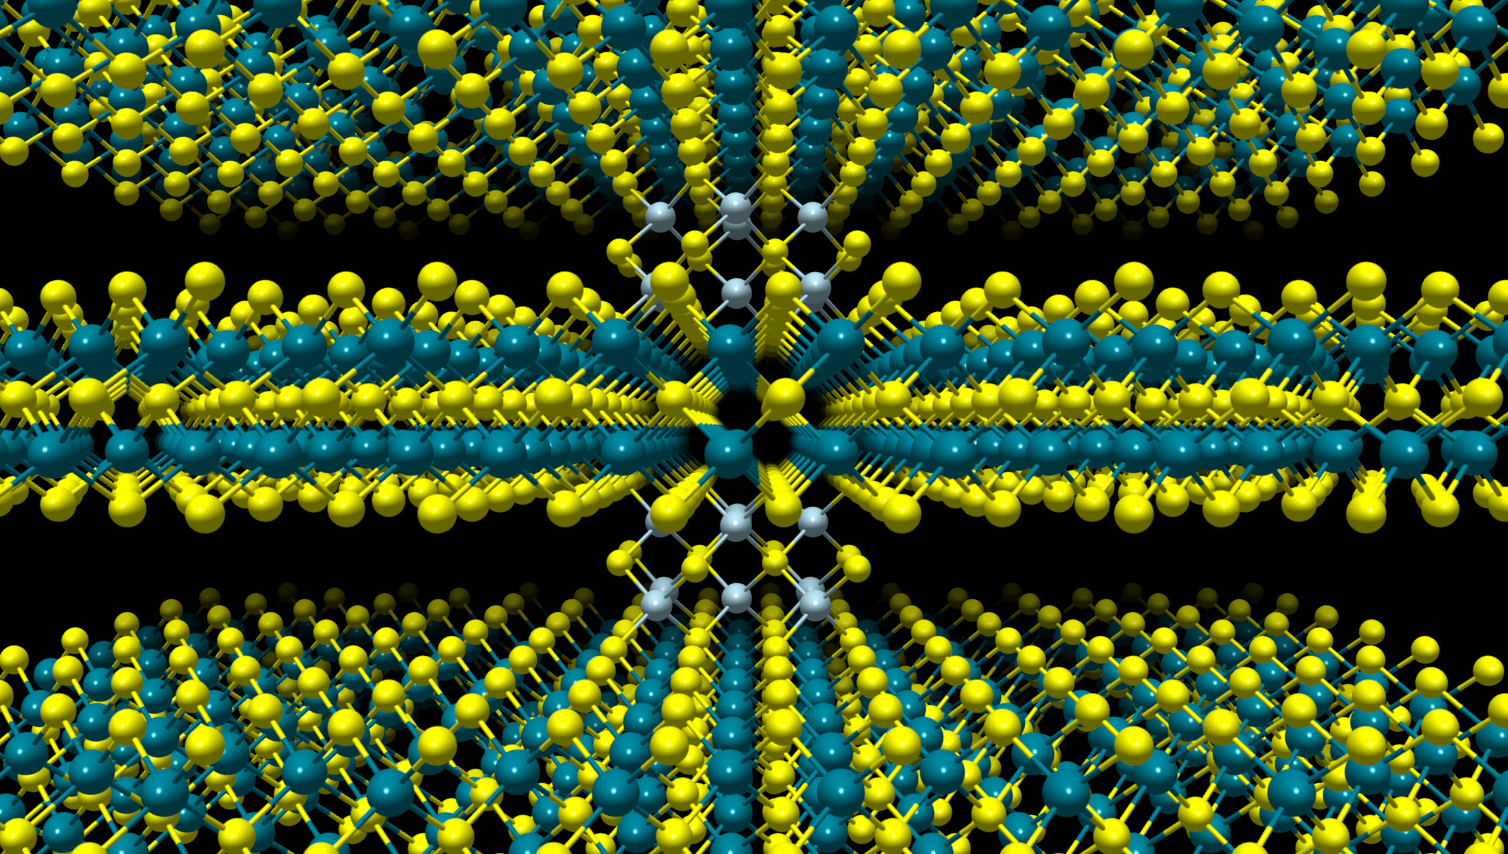
\includegraphics[width=\paperwidth,height=\paperheight]{../beamer-figures/title-page/AlGaAs-back-0-lp}};
     

\node[anchor=north west,
scale=0.08,
inner sep=0pt,
opacity=1,
](iicologo) 
at (current page.north west) {
\includegraphics{../beamer-figures/title-page/logo_iico_azul.png}};

\node[anchor=north east,
scale=0.15,
inner sep=0pt,
opacity=1,
](iicologo) 
at (current page.north east) {
\includegraphics{../beamer-figures/title-page/logo_uaslp_azul.png}};      
     
     
\node[text width=0.65\paperwidth,
      anchor=north,
	inner sep=0pt,
	yshift=-0.5cm,
      align=center,
      scale=1.1] (uni) at (current page.north) { 
   UNIVERSIDAD AUTONOMA DE SAN LUIS POTOSI\\
   FACULTAD DE CIENCIAS\\
   POSGRADO EN CIENCIAS APLICADAS        
       };     
     
%\node[font=\fontsize{14}{10}\selectfont, 
%      text width=17cm,
%      anchor=center,
%      inner sep=0pt,
%      yshift=1.8cm,
%      color=blue!20!black!80,
%      align=center] (title) at (current page.center) { 
%      
%           };
%       
\node[%
%font=\bfseries\fontsize{20}{10}\selectfont, 
text width=0.9\paperwidth,
anchor=center,
inner sep=0pt,
yshift=1cm,
color=blue,
align=center,
scale=2] (title) at (current page.center)  { 
	Pozos Cuánticos Acoplados como una nueva\\
fuente de Anisotropías \'Opticas\\
en Sistemas Nanoestructurados
};
       
\node[below = of title,
text width=0.5\paperwidth,
inner sep=0pt,
yshift=0cm,
align=center,
scale=1.2] (author) {
                        OSCAR RUIZ CIGARRILLO\\
                         };       
       
\node[below = of author,
text width=30cm,
inner sep=0pt,
yshift=0.5,
align=center,
scale=1.1] (profesor) { 
		                {\color{blue}Asesores de tesis} \\
                        Dr. Luis Felipe Lastras Martinez\\
                        Dr. Raul Eduardo Balderas Navarro\\
                        Dr. Edgar Armando Cerda Mendez
                     };   
\node[below = of profesor,
text width=\textwidth,
inner sep=0pt,
yshift=0.5cm,
align=center,
scale=0.7] (date) {SAN LUIS POTOSÍ, MÉXICO, \today};                     
                             
\end{tikzpicture}

\end{titlepage}
\end{frame}



\begin{frame}[t]{Contenido}{}
\tableofcontents
\end{frame}

%============================================ Introduction ================================================
\section{Introducción}
\subsection{Estructura de Bandas}
\begin{frame}[t]
\frametitle{Introducci\'on}
\framesubtitle{Estructura de Bandas}
\vspace{-0.5cm}
\begin{tikzpicture}[remember picture, overlay]
\node<1->[anchor = north west, text width =0.7\textwidth, yshift = -0.75cm](txt) at (current page.north west) {
	\begin{tcolorbox}[enhanced,title =Estructura de Bandas,
	left=1mm,
	top=1mm,
	bottom=1mm,
	right=1mm,
	width =\textwidth,
	height=0.45\textheight,
	boxsep = 0cm,
	coltitle=blue,
	attach boxed title to top center={yshift=-2mm,yshifttext=-1mm},
	boxed title style={colframe=blue,
		colback=gc!90}]
	\begin{itemize}
	\item<1-> Dicta el comportamiento de los electrones dentro de un solido
	\item<2-> En un solido $\approx 10^{23}$ atomos\\$\rightarrow$\text{\color{red}problema complejo de muchos cuerpos}
	\item<3-> Hamiltoniano de un solido
	\item<4-> Gracias al Teorema de Bloch\\ $\rightarrow$ potencial periodico
	\item<5-> Ecuacion de Schr\"odinger en terminos de un el\'ectron. 
	\end{itemize}
	\end{tcolorbox}	
};

% \node<1->[anchor=north east,xshift=-2cm,yshift=-1cm] at (current page.north east){\includegraphics[width=0.35\textwidth]{../../../scripts/structures/GaAs-2}};

\node<3>[anchor=center,text width=\textwidth,font=\sffamily,xshift=-1cm,yshift=-2cm] at (current page.center){
\begin{equation*}
	\begin{split}
	H  =  &\dfrac{1}{2M}\sum\limits_{i=1}^{N_{n}} \bff{P}_{j}^{2} + \dfrac{1}{2m_{0}} \sum\limits_{j=1}^{N_{e}} \bff{p}_{j}^{2} + \dfrac{Z^{2}}{2} \sum\limits_{i,j=1,i\neq j}^{N_{n}} V_{c}\left(\bff{R}_{i}-\bff{R}_{j}\right)-Z\sum\limits_{i=1}^{N_{n}}\sum\limits_{j=1}^{N_{e}}V_{c}\left(\bff{r}_{j}-\bff{R}_{i}\right) \\
	& + \dfrac{1}{2} \sum\limits_{i,j=1,i\neq j}^{N_{e}} V_{c} \left(\bff{r}_{i}-\bff{r}_{j}\right)
	\end{split}
\end{equation*}
};

% \node<4->[anchor=south west,opacity=0.5](i1) at (current page.south west){\includegraphics[width=\textwidth,trim = {0cm 0cm 0cm 2cm},clip]{beamer-figures/introduction/atom-line.png}};
% \node<4->[anchor=center,yshift=0cm,inner sep=0mm,yshift=-0.5cm](bloch) at (i1.center){\animategraphics[autoplay,loop,width=\textwidth]{8}{beamer-figures/introduction/b1}{}{}};

% \node<4->[anchor=south west,text width=\textwidth,scale=0.7] at (current page.south west) {Image credit: from \href{https://commons.wikimedia.org/wiki/File:Standing_wave.gif}{Wikimedia Commons}, public domain};
% \node<5->[anchor=south west,yshift=-0.5cm,inner sep=0mm](schrodinger)at(bloch.north){$\left[-\dfrac{\hbar^2}{2m_{0}}\nabla^2 + U(\rv)\right]\psi (r)=\senergy\psi(\rv)$}; 


\end{tikzpicture}
\end{frame}




% \include{./Files/RESUMEN}
% \include{./Files/NEW-RESULTS}
%\include{./Files/CONCLUSIONS}


{
\aauwavesbg%
\begin{frame}[plain,noframenumbering]%
  \finalpage{\huge \textcolor{blue}{Gracias por su atención!}}
\end{frame}
}

%%%%%%%%%%%%%%%%%%%%%%%%%%%%%%%%%%%%%%%%%%%%%%%%%%%%%%%%%%%%%%%%%%%%%%%%%%%%%%%%%%%%%%%%%%%%%%%%%%

\end{document}
